\documentclass{standalone}
\usepackage{tikz}
\usetikzlibrary{patterns}
\usetikzlibrary{positioning}
\usetikzlibrary{patterns, positioning}
\usetikzlibrary{shapes.misc}
\usepackage[outline]{contour}
\contourlength{1.5pt} 
\usepackage[sfdefault]{ClearSans}

\begin{document}
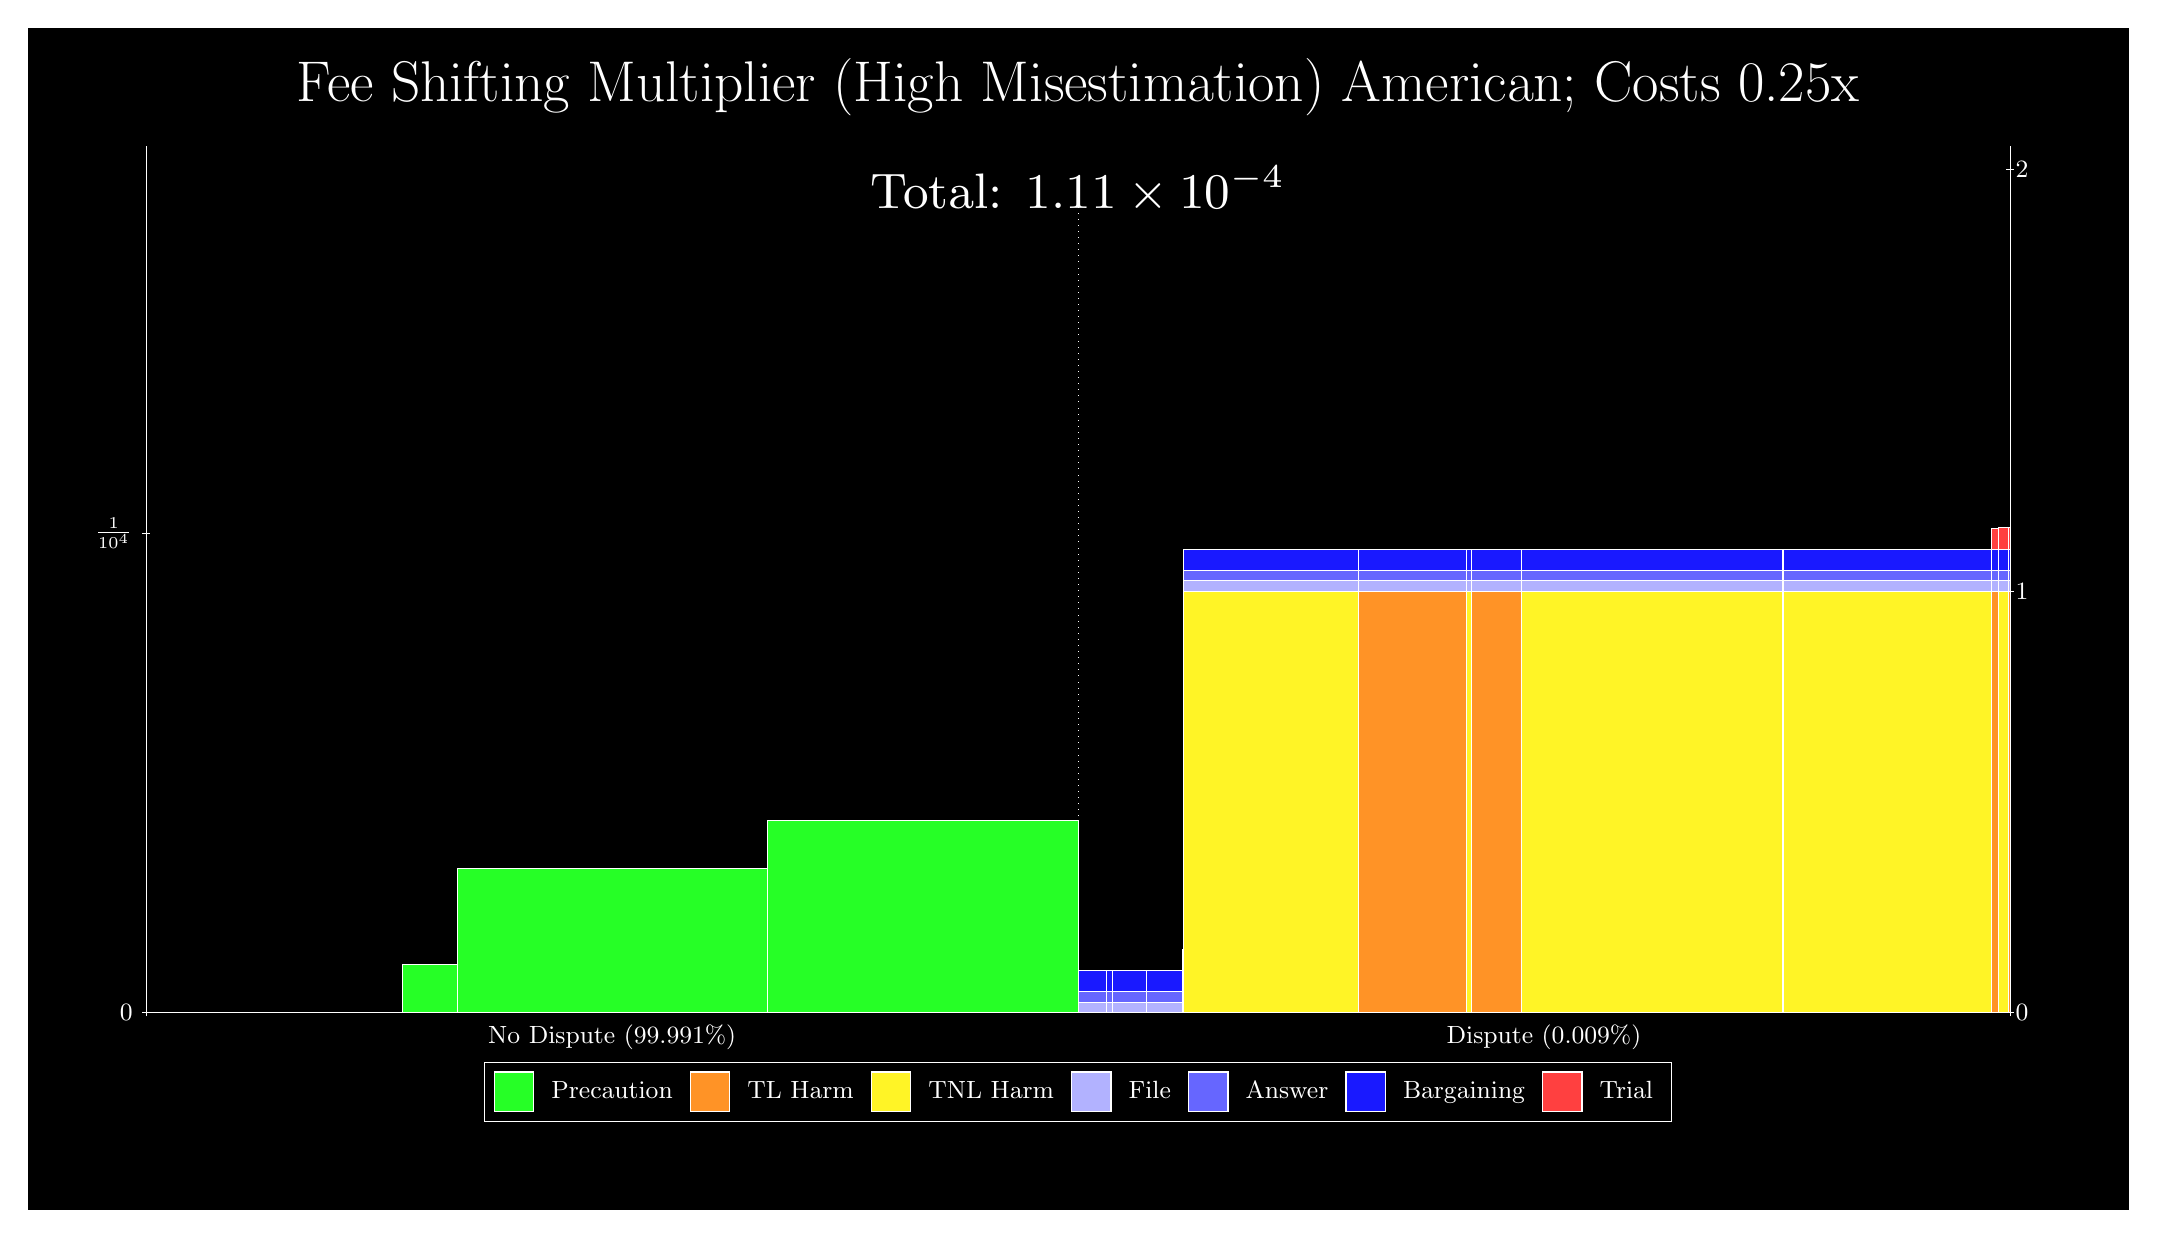
\begin{tikzpicture}
\draw[fill=black] (0,0) rectangle (26.667,15);
\draw[draw=none,text=white] (0,13.5) rectangle (26.667,15) node[midway] {\huge Fee Shifting Multiplier (High Misestimation) American; Costs 0.25x};
\draw[fill=green!85,draw=white,very thin] (4.7447,2.5) rectangle (5.4444,3.1087);
\draw[fill=green!85,draw=white,very thin] (5.4444,2.5) rectangle (9.3888,4.3261);
\draw[fill=green!85,draw=white,very thin] (9.3888,2.5) rectangle (13.333,4.9348);
\draw[fill=blue!30,draw=white,very thin] (13.333,2.5) rectangle (13.693,2.6338);
\draw[fill=blue!60,draw=white,very thin] (13.333,2.6338) rectangle (13.693,2.7676);
\draw[fill=blue!90,draw=white,very thin] (13.333,2.7676) rectangle (13.693,3.0353);
\draw[fill=green!85,draw=white,very thin] (13.693,2.5) rectangle (13.772,2.5001);
\draw[fill=blue!30,draw=white,very thin] (13.693,2.5001) rectangle (13.772,2.6339);
\draw[fill=blue!60,draw=white,very thin] (13.693,2.6339) rectangle (13.772,2.7677);
\draw[fill=blue!90,draw=white,very thin] (13.693,2.7677) rectangle (13.772,3.0353);
\draw[fill=green!85,draw=white,very thin] (13.772,2.5) rectangle (14.199,2.5002);
\draw[fill=blue!30,draw=white,very thin] (13.772,2.5002) rectangle (14.199,2.634);
\draw[fill=blue!60,draw=white,very thin] (13.772,2.634) rectangle (14.199,2.7678);
\draw[fill=blue!90,draw=white,very thin] (13.772,2.7678) rectangle (14.199,3.0354);
\draw[fill=green!85,draw=white,very thin] (14.199,2.5) rectangle (14.65,2.5002);
\draw[fill=blue!30,draw=white,very thin] (14.199,2.5002) rectangle (14.65,2.634);
\draw[fill=blue!60,draw=white,very thin] (14.199,2.634) rectangle (14.65,2.7678);
\draw[fill=blue!90,draw=white,very thin] (14.199,2.7678) rectangle (14.65,3.0355);
\draw[fill=green!85,draw=white,very thin] (14.65,2.5) rectangle (14.671,2.5002);
\draw[fill=blue!30,draw=white,very thin] (14.65,2.5002) rectangle (14.671,2.634);
\draw[fill=blue!60,draw=white,very thin] (14.65,2.634) rectangle (14.671,2.7678);
\draw[fill=blue!90,draw=white,very thin] (14.65,2.7678) rectangle (14.671,3.0354);
\draw[fill=red!75,draw=white,very thin] (14.65,3.0354) rectangle (14.671,3.3031);
\draw[fill=yellow!85,draw=white,very thin] (14.671,2.5) rectangle (16.894,7.8526);
\draw[fill=blue!30,draw=white,very thin] (14.671,7.8526) rectangle (16.894,7.9864);
\draw[fill=blue!60,draw=white,very thin] (14.671,7.9864) rectangle (16.894,8.1203);
\draw[fill=blue!90,draw=white,very thin] (14.671,8.1203) rectangle (16.894,8.3879);
\draw[fill=orange!85,draw=white,very thin] (16.894,2.5) rectangle (18.266,7.8526);
\draw[fill=blue!30,draw=white,very thin] (16.894,7.8526) rectangle (18.266,7.9864);
\draw[fill=blue!60,draw=white,very thin] (16.894,7.9864) rectangle (18.266,8.1203);
\draw[fill=blue!90,draw=white,very thin] (16.894,8.1203) rectangle (18.266,8.3879);
\draw[fill=green!85,draw=white,very thin] (18.266,2.5) rectangle (18.323,2.5001);
\draw[fill=yellow!85,draw=white,very thin] (18.266,2.5001) rectangle (18.323,7.8527);
\draw[fill=blue!30,draw=white,very thin] (18.266,7.8527) rectangle (18.323,7.9865);
\draw[fill=blue!60,draw=white,very thin] (18.266,7.9865) rectangle (18.323,8.1203);
\draw[fill=blue!90,draw=white,very thin] (18.266,8.1203) rectangle (18.323,8.3879);
\draw[fill=green!85,draw=white,very thin] (18.323,2.5) rectangle (18.959,2.5001);
\draw[fill=orange!85,draw=white,very thin] (18.323,2.5001) rectangle (18.959,7.8527);
\draw[fill=blue!30,draw=white,very thin] (18.323,7.8527) rectangle (18.959,7.9865);
\draw[fill=blue!60,draw=white,very thin] (18.323,7.9865) rectangle (18.959,8.1203);
\draw[fill=blue!90,draw=white,very thin] (18.323,8.1203) rectangle (18.959,8.3879);
\draw[fill=green!85,draw=white,very thin] (18.959,2.5) rectangle (22.277,2.5002);
\draw[fill=yellow!85,draw=white,very thin] (18.959,2.5002) rectangle (22.277,7.8528);
\draw[fill=blue!30,draw=white,very thin] (18.959,7.8528) rectangle (22.277,7.9866);
\draw[fill=blue!60,draw=white,very thin] (18.959,7.9866) rectangle (22.277,8.1204);
\draw[fill=blue!90,draw=white,very thin] (18.959,8.1204) rectangle (22.277,8.388);
\draw[fill=green!85,draw=white,very thin] (22.277,2.5) rectangle (22.286,2.5002);
\draw[fill=orange!85,draw=white,very thin] (22.277,2.5002) rectangle (22.286,7.8528);
\draw[fill=blue!30,draw=white,very thin] (22.277,7.8528) rectangle (22.286,7.9866);
\draw[fill=blue!60,draw=white,very thin] (22.277,7.9866) rectangle (22.286,8.1204);
\draw[fill=blue!90,draw=white,very thin] (22.277,8.1204) rectangle (22.286,8.388);
\draw[fill=green!85,draw=white,very thin] (22.286,2.5) rectangle (24.93,2.5002);
\draw[fill=yellow!85,draw=white,very thin] (22.286,2.5002) rectangle (24.93,7.8528);
\draw[fill=blue!30,draw=white,very thin] (22.286,7.8528) rectangle (24.93,7.9866);
\draw[fill=blue!60,draw=white,very thin] (22.286,7.9866) rectangle (24.93,8.1205);
\draw[fill=blue!90,draw=white,very thin] (22.286,8.1205) rectangle (24.93,8.3881);
\draw[fill=yellow!85,draw=white,very thin] (24.93,2.5) rectangle (24.933,7.8526);
\draw[fill=blue!30,draw=white,very thin] (24.93,7.8526) rectangle (24.933,7.9864);
\draw[fill=blue!60,draw=white,very thin] (24.93,7.9864) rectangle (24.933,8.1203);
\draw[fill=blue!90,draw=white,very thin] (24.93,8.1203) rectangle (24.933,8.3879);
\draw[fill=red!75,draw=white,very thin] (24.93,8.3879) rectangle (24.933,8.6555);
\draw[fill=orange!85,draw=white,very thin] (24.933,2.5) rectangle (25.024,7.8526);
\draw[fill=blue!30,draw=white,very thin] (24.933,7.8526) rectangle (25.024,7.9864);
\draw[fill=blue!60,draw=white,very thin] (24.933,7.9864) rectangle (25.024,8.1203);
\draw[fill=blue!90,draw=white,very thin] (24.933,8.1203) rectangle (25.024,8.3879);
\draw[fill=red!75,draw=white,very thin] (24.933,8.3879) rectangle (25.024,8.6555);
\draw[fill=green!85,draw=white,very thin] (25.024,2.5) rectangle (25.148,2.5002);
\draw[fill=yellow!85,draw=white,very thin] (25.024,2.5002) rectangle (25.148,7.8528);
\draw[fill=blue!30,draw=white,very thin] (25.024,7.8528) rectangle (25.148,7.9866);
\draw[fill=blue!60,draw=white,very thin] (25.024,7.9866) rectangle (25.148,8.1204);
\draw[fill=blue!90,draw=white,very thin] (25.024,8.1204) rectangle (25.148,8.388);
\draw[fill=red!75,draw=white,very thin] (25.024,8.388) rectangle (25.148,8.6557);
\draw[fill=green!85,draw=white,very thin] (25.148,2.5) rectangle (25.167,2.5002);
\draw[fill=orange!85,draw=white,very thin] (25.148,2.5002) rectangle (25.167,7.8528);
\draw[fill=blue!30,draw=white,very thin] (25.148,7.8528) rectangle (25.167,7.9866);
\draw[fill=blue!60,draw=white,very thin] (25.148,7.9866) rectangle (25.167,8.1204);
\draw[fill=blue!90,draw=white,very thin] (25.148,8.1204) rectangle (25.167,8.388);
\draw[fill=red!75,draw=white,very thin] (25.148,8.388) rectangle (25.167,8.6557);
\node[font=\small,text=white,anchor=north,scale=2] at (13.333, 13.5) {Total: $1.11\times 10^{-4}$};
\draw[white,very thin] (1.5,2.5) -- (1.5,13.5);
\draw[white,very thin] (1.45,2.5) -- (1.55,2.5);
\node[font=\small,text=white, anchor=east] at (1.45, 2.5) {0};
\draw[white,very thin] (1.45,8.587) -- (1.55,8.587);
\node[font=\small,text=white, anchor=east] at (1.45, 8.587) {$\frac{1}{10^{4}}$};

\draw[white,dotted,very thin] (13.333,2.83) -- (13.333,13.17);
\draw[white,very thin] (25.167,2.5) -- (25.167,13.5);
\draw[white,very thin] (25.117,2.5) -- (25.217,2.5);
\node[font=\small,text=white, anchor=west] at (25.117, 2.5) {0};
\draw[white,very thin] (25.117,7.8526) -- (25.217,7.8526);
\node[font=\small,text=white, anchor=west] at (25.117, 7.8526) {1};
\draw[white,very thin] (25.117,13.205) -- (25.217,13.205);
\node[font=\small,text=white, anchor=west] at (25.117, 13.205) {2};

\draw[white,very thin] (1.5,2.5) -- (25.167,2.5);
\draw[white,very thin] (1.5,2.45) -- (1.5,2.55);
\node[font=\small,text=white, anchor=north] at (1.5, 2.45) {};
\draw[white,very thin] (25.167,2.45) -- (25.167,2.55);
\node[font=\small,text=white, anchor=north] at (25.167, 2.45) {};

\node[font=\small,text=white,anchor=south] at (7.4167, 1.9) {No\ Dispute\ (99.991\%)};
\node[font=\small,text=white,anchor=south] at (19.25, 1.9) {Dispute\ (0.009\%)};
\draw (13.3333,2.5) node (B) {};
\begin{scope}[align=center]
\matrix[scale=0.5,draw=white,below=0.5cm of B,nodes={draw},column sep=0.1cm]{
\node[rectangle,draw,minimum width=0.5cm,minimum height=0.5cm,fill=green!85]{}; & \node[draw=none,font=\small,text=white]{Precaution}; &
\node[rectangle,draw,minimum width=0.5cm,minimum height=0.5cm,fill=orange!85]{}; & \node[draw=none,font=\small,text=white]{TL Harm}; &
\node[rectangle,draw,minimum width=0.5cm,minimum height=0.5cm,fill=yellow!85]{}; & \node[draw=none,font=\small,text=white]{TNL Harm}; &
\node[rectangle,draw,minimum width=0.5cm,minimum height=0.5cm,fill=blue!30]{}; & \node[draw=none,font=\small,text=white]{File}; &
\node[rectangle,draw,minimum width=0.5cm,minimum height=0.5cm,fill=blue!60]{}; & \node[draw=none,font=\small,text=white]{Answer}; &
\node[rectangle,draw,minimum width=0.5cm,minimum height=0.5cm,fill=blue!90]{}; & \node[draw=none,font=\small,text=white]{Bargaining}; &
\node[rectangle,draw,minimum width=0.5cm,minimum height=0.5cm,fill=red!75]{}; & \node[draw=none,font=\small,text=white]{Trial}; \\\\
};\end{scope}

\end{tikzpicture}
\end{document}